\markboth{Photoplethysmography}{Photoplethysmography}

\chapter{Photoplethysmography}
\label{cha:Photoplethysmography}

\section{Physical principle}
\label{sec:Physical principle}
Photoplethysmography (PPG) is an optical technique that measures blood-volume changes.
PPG utilizes optical sensors to detect these changes by emitting light into the skin and measuring the amount of light absorbed or reflected by blood vessels.
Depending on the energy of incident photons, bond deformation or vibration at different energy level of different bonds occurs. So, only the photon with energy 
that corresponds to the difference between two of its energy levels can be absorbed.\cite{azudin_principles_2023, castaneda_review_2018}
Glucose absorbs light at the fundamental frequencies (2–2.5 $ \mu $m) and first overtone region (1.53–1.82 $ \mu $m). These wavelengths have the drawbacks of needing 
expensive sensors, strong absorption due to water and scattering of fatty tissue. For the second overtone region (0.8-1.6 $ \mu $m) on the other hand, way cheaper 
infrared sensors can be used. The absorbance of glucose is much weaker compared to the previously mentioned wavelengths, but still detectable compared to other 
tissue chromophores. \cite{hossain_estimation_2019}

\section{Transmission vs. reflection method}
\label{sec:Transmission vs. reflection method}
There are two implementation for PPG:

\textbf{Transmission PPG} places the light source on one side of a thin body part (e.g., fingertip or earlobe) and the photodetector on the opposite side. This way the light traverses the tissue. This method usually yields a higher amplitude and cleaner waveforms. The drawback is that it requires thin, well-perfused bodyparts and is sensitive to local perfusion changes (e.g., cold-induced vasoconstriction).\cite{castaneda_review_2018}
\begin{figure}[H]
    \centering
    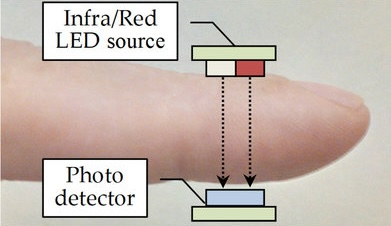
\includegraphics[scale=0.5]{Figures/Transmission_ppg.jpg}
    \caption{Transmission PPG on a finger}
    \label{fig:transmission_ppg}
\end{figure}

\textbf{Reflection PPG} places the light source and photodetector on the same side. The light enters, scatters within the tissue, and a portion of it returns to the photodetector. While the amplitude is often lower and more prone to motion artifact than transmission PPG, reflection PPG works on most body sites.\cite{castaneda_review_2018,azudin_principles_2023}
\begin{figure}[H]
    \centering
    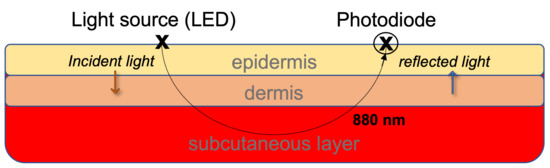
\includegraphics[scale=0.75]{Figures/Reflection_ppg.jpg}
    \caption{Reflection PPG principle}
    \label{fig:reflection_ppg}
\end{figure}

\section{Signal characteristics and challenges}
\label{sec:Signal characteristics and challenges}

\textbf{Physiological content.}  
The PPG signal carries a mix of information. The pulsatile part (AC) reflects stroke volume, arterial stiffness, and wave reflections, which can be seen in its amplitude, rise time, and the shape of the dicrotic notch. Breathing introduces slower variations in the baseline. Taking the second derivative of the PPG makes the inflection points more visible and allows the calculation of indices linked to vascular aging and stiffness.\cite{castaneda_review_2018,azudin_principles_2023}

\textbf{Artifacts and confounders.}  
Several factors can distort the signal: Movement of the sensor or tissue can change how light passes through which creates motion artifacts. Stray ambient light may leak into the sensor. Blood flow at the measurement site can also vary with temperature or autonomic activity. For example, vasoconstriction can reduce or even eliminate the signal at extremeties. The amount of pressure from the device itself matters too, since it alters local blood volume. Peripheral sites are the most affected when perfusion is low, while the ear canal has shown stable signals with fewer dropouts, even during induced vasoconstriction or in surgical conditions.\cite{budidha_human_2014,venema_robustness_2014} To improve signal quality, common steps include subtracting ambient light, adaptive filtering, using motion references for regression, robust peak detection, and applying quality checks before extracting features or feeding the data into models.\cite{castaneda_review_2018,azudin_principles_2023}

\textbf{Implications for body-site choice.}  
Where the sensor is placed strongly affects performance. Transmission PPG usually produces higher amplitudes and cleaner signals but often fail during cold-induced vasoconstriction. Reflection PPG setups can be used at most body sites, but they typically have lower amplitude and are more sensitive to motion.\cite{castaneda_review_2018,azudin_principles_2023,budidha_human_2014,venema_robustness_2014}
